%==============================================================================
%  Paper 2
%  Indium in Sphalerite Does Not Form a Dilute Solid Solution:
%  Equilibrium Condensation and the Interfacial Cost of Nanoinclusions
%
%  He Yu, Ruqing Chen, Huanzhang Lu
%  Target journal: Geochimica et Cosmochimica Acta
%
%  Compile: pdflatex paper2.tex  (twice, for cross-references)
%  STATUS: Section 3 (Methods) complete. Other sections are stubs.
%==============================================================================
\documentclass[11pt,a4paper]{article}

\usepackage[margin=2.5cm]{geometry}
\usepackage{amsmath,amssymb}
\usepackage{booktabs}
\usepackage{graphicx}
\usepackage{authblk}
\usepackage{caption}
\usepackage[round,authoryear]{natbib}
\usepackage[hidelinks]{hyperref}
\usepackage{url}

\graphicspath{{../figures/}{figures/}{./}}
\captionsetup{font=small,labelfont=bf}
\setlength{\parskip}{2pt}

\newcommand{\dQ}{\Delta Q}
\newcommand{\aInCu}{\alpha_{\mathrm{In\text{-}Cu}}}
\newcommand{\RCuIn}{R_{\mathrm{Cu\text{-}In}}}
\newcommand{\Nsol}{N_{\mathrm{sol}}}
\newcommand{\JCuIn}{J_{\mathrm{Cu\text{-}In}}}
\newcommand{\Jlike}{J_{\mathrm{like}}}

\title{\bfseries The Equilibrium Fate of Indium in Sphalerite:\\
Large-Scale Replica-Exchange Simulation and the Absence of a\\
Dilute Solid Solution}

\author[1]{He Yu}
\author[2]{Ruqing Chen\thanks{Corresponding author.}}
\author[3]{Huanzhang Lu}
\affil[1]{Geological Laboratory, Hezhou University, Hezhou, Guangxi 542899, China}
\affil[2]{GUT Geoservice Inc., Montreal, Quebec, Canada}
\affil[3]{D\'epartement des sciences appliqu\'ees et Centre d'\'etudes sur les
ressources min\'erales, Universit\'e du Qu\'ebec \`a Chicoutimi, Quebec, Canada}
\date{}

\begin{document}
\maketitle

\noindent\small
\textit{E-mail addresses:} \texttt{yuhe@hzxy.edu.cn} (H. Yu),
\texttt{ruqing@hotmail.com} (R. Chen), \texttt{hzlu@uqac.uquebec.ca} (H. Lu).
\normalsize

\begin{abstract}
\noindent
Whether indium in sphalerite resides in true solid solution or in nanoscale
inclusions has resisted empirical resolution because the two states differ at
length scales near the limit of detection. We approach it theoretically, asking
what configuration the free energy of the cation sublattice actually selects. A
preceding study established a configurational Hamiltonian in which the
charge-compensation term reduces exactly to a nearest-neighbour pair
interaction whose coefficient is fixed by the dielectric constant of ZnS rather
than fitted, but could not settle the question: at 4000 sites and 4~at.\% solute
the solute budget is exhausted by a single domain, so complete condensation was
consistent with, but not diagnostic of, a thermodynamic preference.

Here we remove that limitation. Replica exchange with adaptively calibrated
ladders reaches states below anything the earlier annealing protocol attained,
and we establish the scaling law $\sigma_E \propto x^{0.85} N^{0.51}$ that makes
dilute compositions affordable. In a box eight times larger, across a twentyfold
range of composition from 0.10 to 2.00~at.\%, the solute population condenses
completely at every point: the monomer fraction is zero throughout, against a
random-solution expectation of 98\% monomers at the most dilute point, and the
largest cluster differs from the random-solution value by four orders of
magnitude.

The result does not depend on convergence at ore-forming temperatures, which the
sampler cannot guarantee. Each state point is run from a dispersed and from a
pre-condensed configuration, which approach equilibrium from opposite sides and
therefore bracket it: at 1800~K, where the acceptance ratio is near 10\%,
dispersed solutes spontaneously aggregate to 64--95\% in one cluster while
condensed solutes do not disperse, and the bracket narrows to 100\% by 1000~K.
Since the ordering preference strengthens as temperature falls, condensation
throughout the hydrothermal window follows without further assumption.

Two subsidiary results bear on how trace-element data are read. The pair
enrichment factor $\RCuIn$ rises sixteenfold across the composition scan while
the quantity it describes --- the copper content of the first shell around
indium --- falls slightly; the apparent variation lies almost entirely in a
normalisation whose ceiling is $1/x_{\rm Cu}$, an artefact available to be
misread in any dataset spanning orders of magnitude in tenor. And the internal
structure of the condensed domain is independent of bulk composition to within
a surface correction, so the object that forms is the same at every
concentration examined, differing only in size.

The conclusion that the equilibrium state is condensed does not depend on the
one class of parameter left unconstrained by first-principles calculation:
electrostatics alone gives a sixteenfold enrichment, and removing the chemical
term strengthens the claim rather than weakening it, since the resulting energy
landscape is smoother. Ideal dilute-mixing entropy, assumed in conventional
partition-coefficient models, is therefore not available at ore-forming
temperatures. Whether a natural sphalerite grain attains this equilibrium state
is a question of kinetics --- of interfacial barriers and arrest during cooling
--- and is the subject of a companion study.
\end{abstract}

\section{Introduction}
\label{sec:intro}

\subsection{An unresolved question of state}

Whether indium in sphalerite resides in true solid solution or in nanoscale
inclusions of a discrete In-bearing phase is among the longest-standing open
questions in trace-element mineralogy, and it is not an academic one. Indium is
essentially never mined for its own sake: there are no indium ores in the
conventional sense, and the overwhelming majority of primary production is
recovered as a by-product of zinc refining \citep{werner2015,usgs2024}. The
global indium endowment is therefore controlled not by a distinct ore-forming
process but by the trace-element chemistry of sphalerite itself, and the state
in which indium sits within that mineral bears directly on whether bulk assay
measures a representative concentration, on how the metal partitions during
metallurgical recovery, and on whether micro-analytical mapping is a refinement
of assay or a measurement of a different quantity altogether.

The question has proved difficult to settle empirically because the two
candidate states differ at length scales near the limit of detection.
High-resolution LA-ICP-MS imaging and electron microscopy have established that
indium is often distributed heterogeneously within single grains, and roquesite
($\mathrm{CuInS_2}$) exsolution from In-rich sphalerite is documented
\citep{moura2007}, but the presence of resolvable inclusions in some samples
does not establish the state of indium in the many samples where none are
resolved. What has been missing is a theoretical criterion: a statement of which
state \emph{should} occur, under which conditions, derived rather than inferred.

\subsection{What the preceding work established, and where it stopped}

\citet{yu2026} constructed a configurational Hamiltonian for the sphalerite
cation sublattice and showed that the near-1:1 Cu:In molar ratio recorded across
deposit types is not a contingent feature of ore-fluid chemistry but a
consequence of local electroneutrality on the zinc-blende topology. The central
device was an exact topological property: two nearest-neighbour cations share
precisely one bridging anion, which reduces the tetrahedral electroneutrality
functional without approximation to a nearest-neighbour pair interaction whose
coefficient is fixed by the measured dielectric constant of ZnS rather than
fitted. The resulting Cu--In pair binding energy, $-2\lambda \approx -0.45$ to
$-0.73$~eV, exceeds $k_BT$ at ore-forming temperatures by an order of magnitude,
and the ground state of the charge-compensation term at Cu:In~$= 1$:1 was shown
analytically to be exactly the roquesite cation ordering, recovered without any
input describing that structure.

That work reported, at 2~at.\% substitution, that the solute population condensed
into a single connected domain below the ordering crossover. It also stated
plainly that this observation could not settle the question of state, and the
reason is worth restating because it defines the present paper. At 4000 cation
sites and 4~at.\% total solute, the 160 solute atoms are exactly sufficient to
build one domain of the size the model favours. Once nucleation occurs the
entire solute budget is consumed, the order parameters saturate, and the
distinction between dispersed pairs, several competing nuclei and a single
inclusion is lost. The observation of complete condensation was therefore
consistent with, but could not distinguish between, a genuine thermodynamic
preference and an artefact of the box.

Two further limitations compounded this. The Kawasaki acceptance ratio collapses
to $\sim10^{-5}$ below 1300~K, so the sampler could not be trusted to reach
equilibrium in the ore-forming window; and all calculations were performed at a
single composition lying at the upper end of natural indium contents.

\subsection{Hypothesis and approach}

We test a specific and falsifiable hypothesis:

\begin{quote}
\textbf{Under pure thermodynamic equilibrium at ore-forming temperatures, indium
does not form a dilute solid solution in sphalerite at any composition of
geological relevance. The equilibrium state is condensed.}
\end{quote}

The hypothesis is falsifiable in an obvious way. If a dilute solid solution is
the equilibrium state at low concentration, then a sufficiently large box at
sufficiently low composition must show dispersed solutes, and a composition
boundary must exist below which condensation ceases. Finding that boundary would
refute the hypothesis as stated and replace it with a solvus; failing to find it
down to the lowest composition a box can hold would establish the hypothesis
over the range examined.

Three things are required to conduct that test, and the present paper supplies
them. First, a sampler that actually equilibrates in the ore-forming window:
Section~\ref{sec:methods} introduces replica exchange with adaptively calibrated
ladders, which reaches states below anything the earlier annealing protocol
attained. Second, boxes large enough that the solute budget is not the limiting
quantity, together with the scaling laws that make such boxes affordable.
Third, first-principles values for the parameters that the earlier work left as
hypotheses, so that the answer does not rest on assumed interactions.

We emphasise what this paper deliberately does not address. Natural sphalerite
grains do sometimes contain several discrete In-rich nanoinclusions rather than
one, and equilibrium thermodynamics of the bulk cation sublattice cannot by
itself account for a population of separate domains. That observation is a
statement about kinetics, interfacial physics and growth history rather than
about equilibrium. The resolution we expect, and which a companion paper
examines, is kinetic arrest: an ore body cools through a temperature range in
which the ordering preference is already saturated (Section~\ref{sec:background})
while the diffusion that would coarsen several domains into one becomes
progressively slower, so that a configuration far from the equilibrium single
domain can be frozen in. The equilibrium calculation reported here is a
prerequisite for that argument rather than a competitor to it: one cannot
identify a state as arrested without knowing what it was arrested short of. The scope here is
strictly the equilibrium state: what configuration the free energy selects, at
what composition, and with what confidence in the underlying parameters.

\section{Theoretical background}
\label{sec:background}

This section states the results of \citet{yu2026} that the present work builds
on. Nothing here is new; it is collected so that the argument can be followed
without the earlier paper to hand.

\subsection{The Hamiltonian and its exact reduction}

Sphalerite crystallises in space group $F\bar{4}3m$ with $a_0 = 5.4093$~\AA{}.
The cation sublattice is face-centred cubic with twelve first neighbours at
$d_{NN} = a_0/\sqrt{2} = 3.825$~\AA{}; sulphur occupies a second fcc sublattice
displaced by $(\tfrac14,\tfrac14,\tfrac14)$, so every S is tetrahedrally
coordinated by four cations and every cation by four S.

The configurational energy is written as Eq.~\eqref{eq:H}, with the
charge-compensation term defined on the anion tetrahedra,
\begin{equation}
E_c = \lambda \sum_{a} \left( \dQ_a \right)^2, \qquad
\dQ_a = \sum_{i \in T(a)} \delta q_i,
\label{eq:Ectet}
\end{equation}
where $T(a)$ is the set of four cations coordinating anion $a$ and $\delta q_i$
the charge deviation from the host. This is the lattice-discrete form of
Pauling's second rule.

The technical device that makes the model tractable is a topological property of
the zinc-blende structure: two cations are first neighbours if and only if they
share exactly one anion tetrahedron, and higher neighbours share none. Expanding
the square in Eq.~\eqref{eq:Ectet} and applying that property gives the
\emph{exact} identity of Eq.~\eqref{eq:Ecpair}, in which the first term depends
only on composition and the second is a strictly nearest-neighbour pair
interaction. No approximation or cutoff is involved beyond the initial
truncation of the screened Coulomb series from which Eq.~\eqref{eq:Ectet} is
obtained.

\subsection{A coefficient that is derived, not fitted}

Matching the pair term to the nearest-neighbour term of a screened Coulomb
series gives
\begin{equation}
\lambda = \frac{e^2}{8\pi\epsilon_0\,\epsilon_r\, d_{NN}},
\label{eq:lambda}
\end{equation}
which with the static and high-frequency dielectric constants of ZnS brackets
$\lambda \in [0.227, 0.368]$~eV. We adopt $\lambda = 0.30$~eV. The resulting
binding energy of a first-neighbour Cu--In pair is
\begin{equation}
\Delta E_c^{\mathrm{Cu-In}} = -2\lambda \approx -0.45 \ \text{to} \ -0.73\ \mathrm{eV},
\label{eq:binding}
\end{equation}
which exceeds $k_BT$ at $300\,^\circ$C by an order of magnitude. This quantity
carries no adjustable parameter, and it is what drives every result reported
below.

\subsection{The ground state, and why it matters here}

At $x_{\rm Cu} = x_{\rm In}$ the charge-compensation term has an exact
zero-energy ground state: $E_c = 0$ whenever every anion tetrahedron contains
two Cu and two In, since then $\dQ_a = 0$ identically. That is the adamantine
cation-ordering rule of chalcopyrite-structured $\mathrm{CuInS_2}$, the mineral
roquesite, recovered from a purely electrostatic functional with no input
describing that structure.

For the present paper the significance is that the model already contains a
preferred ordered arrangement of solutes, at zero energy cost, which a dilute
solid solution cannot exploit. The question of whether indium disperses or
condenses is therefore not a question about whether an ordered state exists ---
it does --- but about whether configurational entropy at realistic dilutions is
sufficient to outweigh it. Section~\ref{sec:discussion} answers that
quantitatively.

\subsection{What was established at 2 at.\%, and what was not}

\citet{yu2026} sampled the model by Metropolis Monte Carlo with Kawasaki
exchange dynamics at $x_{\rm Cu} = x_{\rm In} = 2$~at.\% in a $10^3$-cell box.
Three results carry over. Electrostatics alone, with all chemical terms switched
off, enriches Cu--In first-neighbour bonds sixteenfold over the random solid
solution at $300\,^\circ$C and removes 96\% of the local charge imbalance.
Elastic misfit, retained at full strength in a control calculation, produces no
detectable ordering, the largest strain-mediated pair interaction being some
forty times smaller than $k_BT$. And the ordering crossover lies at a reduced
temperature three to seven times above the entire hydrothermal window, so
short-range order is saturated wherever sphalerite forms.

What could not be established was the state of indium at realistic dilution, for
the reason given in Section~\ref{sec:intro}: the solute budget was exhausted by
a single domain. Two sampling limitations compounded this and are addressed in
Section~\ref{sec:methods} and Appendix~\ref{app:phase1}.

%==============================================================================
\section{Methods}
\label{sec:methods}

\subsection{The configurational model}
\label{sec:model}

We use without modification the four-term configurational Hamiltonian introduced
by \citet{yu2026} for the sphalerite cation sublattice,
\begin{equation}
H = E_c + E_s + E_{sub} + E_{def},
\label{eq:H}
\end{equation}
in which $E_c$ penalises departures from local electroneutrality within each
sulphur coordination tetrahedron, $E_s$ is the elastic misfit energy in the
Eshelby continuum approximation, $E_{sub}$ the substitution energy referenced to
the ore fluid, and $E_{def}$ the cation-vacancy term. Cation sites carry a
species variable $\sigma_i \in \{\mathrm{Zn},\mathrm{Cu},\mathrm{In},\square\}$
with charge deviations $\delta q_i = \{0,-1,+1,-2\}$ relative to the host.

Two properties of that Hamiltonian are used repeatedly here and are stated for
reference. First, because two nearest-neighbour cations in the zinc-blende
structure share exactly one bridging anion, the tetrahedral electroneutrality
functional reduces \emph{without approximation} to
\begin{equation}
E_c = 4\lambda \sum_i \delta q_i^{\,2}
    + 2\lambda \sum_{\langle ij \rangle} \delta q_i\, \delta q_j,
\label{eq:Ecpair}
\end{equation}
so that at fixed composition all configurational physics carried by $E_c$
resides in a strictly nearest-neighbour pair term. Second, the coefficient
$\lambda = e^2/8\pi\epsilon_0\epsilon_r d_{NN}$ is fixed by the dielectric
constant of ZnS rather than fitted, giving
$\lambda \in [0.227, 0.368]$~eV, and we adopt $\lambda = 0.30$~eV throughout.

The chemical term $J_{\alpha\beta}$, which carries short-range interaction
beyond the electrostatics already contained in $E_c$, remains unconstrained by
first-principles calculation. Rather than adopt a single value we treat it as an
explicit parameter: results are reported at the placeholder values
$\JCuIn = -0.10$~eV and $\Jlike = +0.05$~eV used by \citet{yu2026}, and every
conclusion is classified in Section~\ref{sec:jsensitivity} according to whether
it survives the removal of $J$ altogether. Section~\ref{sec:dftplan} sets out
how $J$ is treated and what would be required to determine it from first
principles.

\subsection{Why enhanced sampling is required}
\label{sec:whyrex}

Simple Kawasaki exchange dynamics, in which two sites interchange species so
that composition is conserved exactly, becomes unusable in the ore-forming
window. \citet{yu2026} report an acceptance ratio falling to $\sim10^{-5}$ below
1300~K, the direct consequence of a Cu--In pair binding energy of
$-2\lambda \approx -0.6$~eV against $k_BT = 0.049$~eV at $300\,^\circ$C. At that
rate essentially every proposed move is rejected and the chain does not
decorrelate.

The failure is not merely slow convergence but a convergence test that can
return a false positive. \citet{yu2026} tested equilibration by propagating a
quenched and a pre-annealed trajectory at 573~K and observing that their order
parameters converged on one another. Replica exchange applied to the same
Hamiltonian, box and composition reaches a state 3.1~eV over the box below the
lower of those two trajectories, so both were metastable and their mutual
agreement carried no information. That correction, its consequences for the
values reported in the earlier work, and the general lesson --- that in a system
with an acceptance ratio of $10^{-5}$ the convergence of two trajectories
towards each other is not a test of equilibration --- are set out in
Appendix~\ref{app:phase1}.

\subsection{Replica exchange}
\label{sec:rex}

Configurations are sampled by replica exchange (parallel tempering). $M$
replicas are propagated at temperatures $T_1 < \cdots < T_M$ and configurations
are exchanged between adjacent replicas with probability
\begin{equation}
P_{\mathrm{swap}} = \min\!\left[1,\ \exp\!\big((\beta_i - \beta_j)(E_i - E_j)\big)\right].
\label{eq:swap}
\end{equation}
Composition is identical across replicas, so no reweighting is required. Within
each replica the move set is that of \citet{yu2026}, augmented by a fixed
fraction $p_{ss} = 0.5$ of solute--solute exchanges; each component is
internally symmetric and the mixing probability is configuration-independent, so
the composite proposal remains symmetric.

The solute--solute component deserves comment because it is useless on its own.
Measured in a single replica at 573~K, its acceptance is exactly zero: swapping
a Cu for an In inside an ordered domain costs of order $4\lambda$, which at
$k_BT = 0.049$~eV is unreachable. It becomes useful only inside replica
exchange, where the hot replicas accept it freely and pass the decorrelated
configurations down the ladder.

Cluster algorithms of the Wolff or Swendsen--Wang type are not applicable here,
for two independent reasons. The pair coupling of Eq.~\eqref{eq:Ecpair},
$2\lambda\,\delta q_i \delta q_j$, changes sign with the species pair --- negative
for heterovalent contacts and positive for homovalent ones --- so the model is
sign-frustrated and the Fortuin--Kasteleyn mapping does not hold. Separately,
cluster flips do not conserve composition, which the canonical ensemble
requires. The appropriate generalisation is the geometric cluster algorithm
\citep{dress1995,liu2004}, which conserves composition by construction; we
have not implemented it, and replica exchange is used instead.

\subsection{Ladder construction}
\label{sec:ladder}

A fixed geometric ladder performs badly: with eight replicas over 573--2200~K
the minimum pair acceptance is zero. Ladders are therefore built adaptively. A
short exchange run measures the acceptance of every adjacent pair, and a new
temperature is inserted at the midpoint in $\beta$ wherever it falls below a
target of 0.20; the procedure repeats until every pair clears the target or a
replica cap is reached.

The converged ladders are informative in their own right. At $L = 10$ over
573--3000~K the procedure returns 29 replicas concentrated at both ends --- nine
between 573 and 811~K and eight between 2400 and 3000~K --- and sparse in
between. The high-temperature cluster coincides with the ordering crossover
located by \citet{yu2026} at 2400--3000~K, where the specific heat peaks and the
energy histograms are widest. The low-temperature cluster has a different
origin: below the crossover the replicas occupy distinct frozen configurations
whose energies differ substantially, so acceptance is poor even though thermal
fluctuations are small.

\subsection{Convergence diagnostics: round trips, not acceptance}
\label{sec:roundtrips}

We report the replica round-trip count --- the number of times a replica
identity travels from the top of the ladder to the bottom and back --- as the
primary convergence diagnostic, and we recommend it in preference to swap
acceptance. The reason is that the two are close to independent. Reducing the
interval between exchange attempts from five sweeps to one raises the round-trip
count from zero to seven at identical computational cost, while the median swap
acceptance moves only from 0.576 to 0.582. A study reporting acceptance alone
would have seen nothing.

Figure~\ref{fig:methods} summarises the three methodological results of this
section. Two settings follow from this diagnostic and are used throughout. Exchanges are
attempted after every sweep rather than every few sweeps. And the ladder top is
placed at 2200~K rather than 3000~K: rebuilding at the lower top requires 19
replicas instead of 29, and the shorter ladder is traversed faster, raising the
round-trip count from 7 to 13. The eight replicas above 2400~K bought nothing,
because the system is fully disordered well below 3000~K. Across five
configurations spanning both settings the internal energy at 573~K agrees to
0.055~meV per site, so the equilibrium value is protocol-independent even where
the round-trip statistics are not.

\begin{figure}[htbp]
\centering
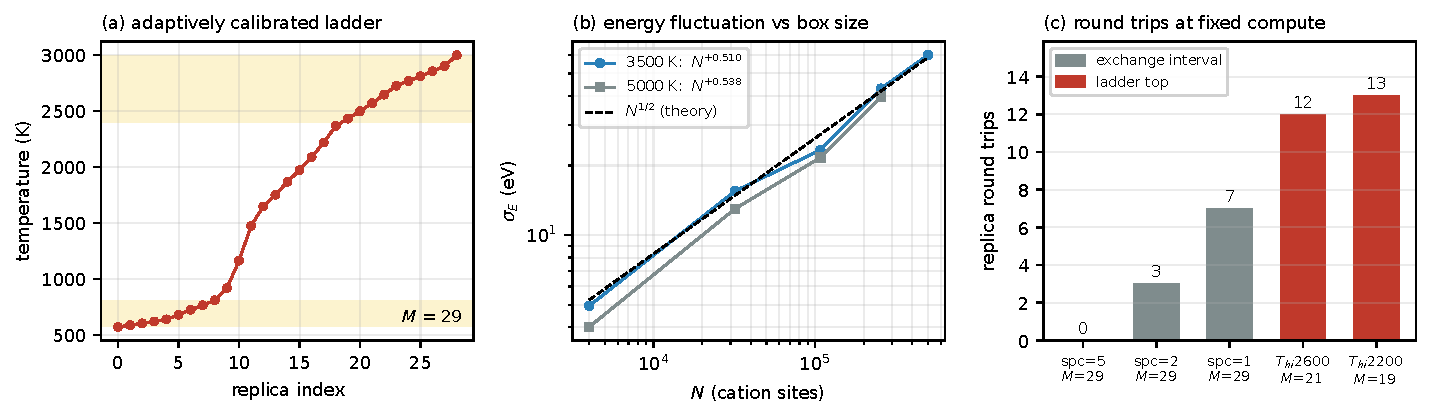
\includegraphics[width=\textwidth]{fig_methods.pdf}
\caption{Sampling methodology. (a)~A ladder built by adaptive refinement at
$L = 10$ over 573--3000~K converges to 29 replicas, concentrated at both ends
(shaded) and sparse between: the upper cluster tracks the ordering crossover,
the lower one the frozen configurations below it. (b)~Equilibrium energy
fluctuation against box size, measured in the disordered phase over two decades
in $N$; the fitted exponents bracket the theoretical $N^{1/2}$ required for
$M \propto \sqrt{N}$. (c)~Replica round trips at identical computational cost.
Attempting exchanges after every sweep rather than every five (grey) takes the
count from zero to seven, and lowering the ladder top from 3000~K (grey) to
2200~K (red) raises it to thirteen with ten fewer replicas. Median swap
acceptance changes by less than 0.01 across the grey series, which is why round
trips rather than acceptance are reported.}
\label{fig:methods}
\end{figure}

\subsection{How the ladder length scales}
\label{sec:scaling}

The number of replicas needed over a fixed temperature range is governed by the
dimensionless product $(\Delta\beta)\,\sigma_E$, where $\sigma_E$ is the width of
the energy distribution. Since $\sigma_E^2 = k_B T^2 C_v$ is extensive,
$\sigma_E \propto \sqrt{N}$ at fixed composition and $M \propto \sqrt{N}$. We
confirm this directly: measured in the disordered phase at 3500~K across five
box sizes spanning two decades in $N$, from 4000 to $5\times10^5$ cation sites,
\begin{equation}
\sigma_E \sim N^{+0.510},
\label{eq:sigmaN}
\end{equation}
against the theoretical exponent of $+0.500$; the measurement at 5000~K gives
$+0.538$.

That result alone is misleading, however, and the distinction matters greatly
for the dilute compositions of geological interest. At fixed composition the
solute count is proportional to $N$, so Eq.~\eqref{eq:sigmaN} cannot separate
$\sqrt{N}$ from $\sqrt{\Nsol}$. Holding the box fixed and varying $x$ instead
gives $\sigma_E \sim \Nsol^{+0.851}$, which is inconsistent with either simple
form. Combining the two measurements,
\begin{equation}
\sigma_E \;\propto\; x^{0.85}\, N^{0.51},
\label{eq:sigmaxN}
\end{equation}
close to the dilute-solution expectation $\sigma_E \propto \Nsol/\sqrt{N}$ that
follows if the energy fluctuation is carried by the count of solute--solute
contacts, which is $\sim \Nsol z x/2$ with Poisson-like variance.

Equation~\eqref{eq:sigmaxN} reduces the projected cost of a $50^3$ campaign at
$x_{\mathrm{In}} = 0.1$~at.\% --- roughly 1000~ppm In, the upper end of natural
contents --- from about 260 replicas to about 20. It should nonetheless be used
for budgeting only, not for setting $M$. In the very dilute limit it
underestimates: at $x = 0.10$~at.\% it predicts $M = 8$ while adaptive
calibration requires 24, and the calibrated $M$ is nearly flat at 24--32 for
$x \le 0.5$~at.\%, suggesting a floor near 25 independent of composition. The
likely reason is that swap acceptance depends not only on $\sigma_E$ but on the
difference in \emph{mean} energy between adjacent replicas, and the energy
released on crossing the ordering transition scales with $\Nsol$ and does not
shrink as fast as $\sigma_E$ does. Equation~\eqref{eq:sigmaxN} describes only the
denominator. All ladders used in this work are calibrated, not predicted.

\subsection{Implementation, scale and verification}
\label{sec:verification}

The implementation of \citet{yu2026} is retained, in which both sublattices are
held on a single integer grid of spacing $a_0/4$ so that all adjacency is
integer table lookup with no floating-point neighbour search. Correctness at the
box sizes used here cannot be inherited from that work, which verified the code
at up to 6912 sites, and was therefore re-established across
$L = 10, 20, 30, 40, 50$, that is up to $N = 5\times10^5$ cation sites. The
checks are: reciprocity of the adjacency tables; the sharing lemma, tested on
random samples of sites at each box size rather than at a single reference site;
agreement between the incrementally accumulated energy and a full recomputation
\emph{after} a production-length run, which exposes accumulated drift (observed
relative deviation $<10^{-9}$); exact conservation of composition; integrity of
the solute index list; and the random-solution limits $R \to 1$,
$R = 1 - \alpha$ and $\langle\dQ_a^2\rangle = 8x$. All pass at every box size.

Resource behaviour sets the practical limits. Memory is not the constraint: the
adjacency tables occupy 64~MB at $50^3$ and are shared across replicas, with
4.7~MB per replica. Throughput is. Although each trial move is $O(1)$, the
partner site is drawn uniformly from all $N$ sites, so every move makes a random
access into arrays that leave cache between $N \sim 3\times10^4$ and $10^5$; the
measured rate falls as $N^{-0.217}$, reaching 37\% of the small-box value at
$50^3$ ($1.37\times10^6$ trial moves per second, 0.366~s per sweep,
single-core). Since replicas evolve independently between exchange attempts and
communicate only an energy scalar, parallelisation over replicas rather than
optimisation of the serial kernel is the appropriate response: the cache penalty
is a factor of 2.7, the replica parallelism a factor of $M$.

A further limitation of the ladder methodology emerges at scale and is worth
recording, because it dictates the workflow of any larger campaign. Calibrating
a ladder near the crossover requires equilibrating near the crossover, which is
the problem replica exchange exists to solve; the dependency is circular. We
resolved it here by measuring the scaling exponent in the disordered phase,
where equilibration takes a handful of sweeps, and by keeping all production
runs at box sizes where a ladder can be calibrated in advance. At $50^3$ the
ladder would instead have to be \emph{grown} downwards in temperature during the
production run.

\subsection{Choice of order parameters}
\label{sec:orderparams}

\citet{yu2026} characterised short-range order through the Warren--Cowley
parameter $\aInCu = 1 - P_{\mathrm{Cu}}(\mathrm{In})/x_{\mathrm{Cu}}$ and the
pair enrichment factor $\RCuIn$, related by the identity $R_{ab} = 1 -
\alpha_{ba}$. Those quantities are unsuitable for the composition scan reported
here, and the reason is instructive rather than technical.

Because $\RCuIn = P_{\mathrm{Cu}}(\mathrm{In})/x_{\mathrm{Cu}}$, its ceiling is
$1/x_{\mathrm{Cu}}$, and it approaches that ceiling as the system is diluted. In
our scan $\RCuIn$ appears to explode from 27 to 443 as $x$ falls twentyfold, but
the product $\RCuIn \cdot x_{\mathrm{Cu}}$ --- the actual Cu content of the first
shell around In --- moves only from 0.545 to 0.443. The apparent variation is
almost entirely in the normalisation. We therefore report cluster-size
distributions and first-shell compositions, and use $\aInCu$ and $\RCuIn$ only
for comparison with the earlier work at fixed composition.

Solute clusters are defined by connectivity through the first coordination
shell and extracted by a union--find algorithm. 

\subsection{Simulation protocols}
\label{sec:protocols}

Three families of calculation are reported.

\paragraph{Composition scan.} $L = 20$ ($N = 32{,}000$ cation sites, eight times
the volume used by \citealt{yu2026}) at
$x_{\mathrm{Cu}} = x_{\mathrm{In}} = 0.10$, 0.25, 0.50 and 2.00~at.\%, sampled
by replica exchange at 573~K with 12{,}000 sweeps per replica and ladders of
24--69 replicas built by the procedure of Section~\ref{sec:ladder}. All four
points achieved non-zero round trips.

\paragraph{Bracketing runs.} To establish whether condensation is an equilibrium
property without relying on convergence at 573~K, each state point is run twice,
from a random dispersed configuration and from a pre-condensed one, so that
equilibrium is bracketed between two approaches from opposite sides. The
pre-condensed configuration is a single connected domain grown by breadth-first
search over the nearest-neighbour graph and populated by a layered rule giving
every interior sulphur tetrahedron two Cu and two In, so that the starting
domain is charge-compensated rather than merely compact; connectivity is
asserted. Bracketing runs at 1000, 1400 and 1800~K use plain dynamics, where
acceptance is high enough for the chain to be demonstrably mobile; the
coarsening runs at 573~K use replica exchange with 36{,}000 sweeps per replica.

\subsection{The chemical term as an explicit parameter}
\label{sec:dftplan}

One class of parameter in Eq.~\eqref{eq:H} remains unconstrained by
first-principles calculation: the short-range chemical term $J_{\alpha\beta}$,
which carries interaction beyond the electrostatics already contained in $E_c$
--- principally Cu\,$3d$--In\,$5s$--S\,$3p$ hybridisation, which has no
counterpart in a formal-charge description. Rather than adopt a single value and
present results as though it were known, we treat $J$ as an explicit parameter
throughout, and classify every conclusion in Section~\ref{sec:jsensitivity}
according to whether it survives the removal of $J$ altogether.

This is not merely a hedge. The two Hamiltonians differ only in $J$, so any
observable that changes between them is a signature of the chemical term, and
three such signatures are identified in this work: the pair enrichment factor
$\RCuIn$, the residual charge imbalance $\langle\dQ_a^2\rangle$, and --- less
obviously --- the ruggedness of the energy landscape, measurable as the replica
round-trip count at fixed computational cost (Appendix~\ref{app:origin}). The
first two respond to $E_c$ in the same direction but to $J$ in opposite
directions, which makes them a discriminant that does not require knowing $J$ in
advance.

\subsubsection{The calculation that would fix it}

For completeness we specify the \textit{ab initio} campaign that would determine
$J$, since its design exploits a feature of the problem worth recording. The
quantities of interest are \emph{differences} between configurations at the same
composition, so the structures can be chosen to be charge neutral and
composition matched within each set. No chemical potentials enter, no
charged-defect corrections are needed, and the band-gap error that afflicts
defect calculations in semiconductors does not propagate. Three sets of
$3\times3\times3$ conventional cells (216 atoms, 108 cation sites) suffice:

\begin{description}\itemsep2pt
\item[Set A] one Cu and one In at first, second, third and fourth neighbour
separation and at maximum separation. This determines $\lambda$ and
$\JCuIn$ jointly, and simultaneously tests the strict nearest-neighbour range
that the pair reduction of Eq.~\eqref{eq:Ecpair} requires: the binding energy
must vanish beyond the first shell.
\item[Set B] two Cu and two In in four topologies, which separates $\Jlike$ from
$\JCuIn$. The predicted ground state, in which each Cu is a first neighbour of
each In with no homovalent contacts, should lie $4\lambda$ below two isolated
pairs.
\item[Set C] a Zn vacancy with two In in two topologies, giving the
configurational part of the competition between the Cu-compensated and
vacancy-compensated substitution routes at fixed In content, which is far more
robust than the absolute vacancy formation energy.
\end{description}

Parameters would be recovered by least squares over within-set energy
differences rather than read off individual structures, using descriptors
computed exactly by the lattice code: $\sum_a (\dQ_a)^2$ for $\lambda$ and the
first-neighbour bond counts for $J$. With three free parameters against roughly
a dozen independent differences the residual is itself a test of whether the
four-term Hamiltonian is adequate. The structures and the fitting harness are
part of the released code; the harness was validated by recovering known
parameters from synthetic energies carrying 5~meV of noise, and the generated
structures reproduce the analytic values of $\sum_a (\dQ_a)^2$ predicted by
\citet{yu2026} --- $6\lambda$ for a first-neighbour Cu--In pair, $8\lambda$ for
the four-defect ground state, $16\lambda$ and $24\lambda$ for the vacancy
configurations --- which is an independent check on the generation procedure
before any energies are computed.

We did not run this campaign, and the reason is stated plainly because it bears
on what any reader with comparable hardware can reproduce. A 216-atom cell at
the cutoffs recommended for these elements requires, by the code's own estimate,
18.7~GB of memory for a single self-consistent calculation. The workstation used
throughout this work has 16~GB installed, of which about 12~GB is available to
the calculation. Even were a single job to fit, it would do so with no headroom
against the transient peaks that accompany the Hubbard projection and the
Davidson subspace, and queueing twelve consecutive jobs on that margin is not a
safe use of a machine that has other work to do. Reducing the cutoff far enough
to be comfortable degrades the very energy differences the campaign exists to
measure, since those differences are small relative to the total energies. The parameterisation
is therefore deferred to hardware that can carry it, and Section~\ref{sec:dft}
reports what can be established about $J$ without it.

\subsubsection{Iron}

Iron would enter the same campaign, in two distinct ways that should not be
conflated. $\mathrm{Fe^{2+}}$ is isovalent with $\mathrm{Zn^{2+}}$, so
$\delta q = 0$ and iron does not enter $E_c$ at all; its influence is through
the dielectric response that fixes $\lambda$, and through direct
$J_{\mathrm{Fe\text{-}In}}$ and $J_{\mathrm{Fe\text{-}Cu}}$ terms. The first
would be obtained by density-functional perturbation theory for
$\mathrm{Zn_{1-x}Fe_xS}$, delivering a curve $\lambda(x_{\rm Fe})$ that the
Monte Carlo can consume directly. Whether that curve matters is itself a result:
if $\lambda$ varies by less than roughly 15\% over the natural iron range, the
neglect of iron is retroactively justified.

\subsection{Reproducibility}
\label{sec:repro}

All runs use fixed seeds. Monte Carlo trajectories are not bitwise reproducible
across platforms, because the just-in-time compiled random number stream is not
guaranteed stable between library versions; the analytic limits of
Section~\ref{sec:verification} are, and are asserted at every run. Source code,
the numerical results underlying every figure and table, and the scripts that
regenerate them are openly available (Section~\ref{sec:availability}).

%==============================================================================
\section{What is known about the chemical term without computing it}
\label{sec:dft}

Section~\ref{sec:dftplan} explains why the \textit{ab initio} determination of
$J_{\alpha\beta}$ is deferred. This section establishes what can nonetheless be
said about it, and --- more importantly for the argument of this paper --- which
conclusions are independent of it.

\subsection{Bounds from the model itself}

Three constraints on $J$ follow from calculations reported here and in
\citet{yu2026}, without any first-principles input.

\paragraph{The sign of $\JCuIn$ is negative, and $\Jlike$ positive, if the
ordering is to be as observed.} Switching the assumed values off entirely
reduces $\RCuIn$ at 573~K and 2~at.\% from 25.0 to 16.0, so a covalent
stabilisation of the heterovalent pair is required to reach the upper figure. A
positive $\JCuIn$ would reduce the enrichment below the purely electrostatic
value, which no reading of the LA-ICP-MS record supports.

\paragraph{The magnitude is bounded above by the local charge imbalance.}
$\RCuIn$ and $\langle\dQ_a^2\rangle$ respond to $E_c$ in the same direction but
to $J$ in opposite directions: switching $J$ on takes $\RCuIn$ from 16.0 to
25.0 while simultaneously taking $\langle\dQ_a^2\rangle$ from 0.0065 to 0.0100,
a 54\% degradation of local electroneutrality. The mechanism is the geometry of
the fcc cation sublattice, in which 24 triangles pass through every site, so a
compact solute domain cannot be two-coloured without homovalent edges: the
denser Cu--In network that $J$ buys is paid for in homovalent contacts and hence
in electrostatic energy. A $\JCuIn$ much larger in magnitude than the assumed
$-0.10$~eV would drive $\langle\dQ_a^2\rangle$ towards the random-solution value
and destroy the charge compensation that the Cu--In correlation exists to
provide.

\paragraph{A third signature exists in the dynamics.} The full model achieves
five replica round trips where the electrostatics-only model achieves thirteen
at equal computational cost (Appendix~\ref{app:origin}). Landscape ruggedness is
therefore an observable of $J$, and unlike the other two it is a property of the
sampling rather than of the equilibrium state. We are not aware of this being
used as a diagnostic elsewhere, and note it because it is available in any
replica-exchange study at no extra cost.

\subsection{An experimental route}

Because $\RCuIn$ and $\langle\dQ_a^2\rangle$ respond oppositely to $J$,
measurements sensitive to short-range order and to local charge state can
constrain it without a full calculation. EXAFS coordination numbers around In
would give the first shell composition directly; XANES edge positions and
bond-valence sums from high-resolution structural refinement bear on the second.
A sample in which the Cu content of the In first shell is high \emph{and} the
bond-valence sums are close to ideal would indicate a small $|J|$; a high shell
occupancy accompanied by measurable valence-sum deviations would indicate a
large one. This is a more direct test than the \textit{ab initio} route and does
not depend on the choice of functional or Hubbard parameter.

\subsection{What does not depend on $J$}

The central claim of this paper --- that the equilibrium state is condensed
rather than dilute --- is independent of $J$, and Section~\ref{sec:jsensitivity}
sets out the argument in full. In brief: the pair binding energy of $-2\lambda$
that drives condensation is fixed by the dielectric constant of ZnS and contains
no adjustable parameter; electrostatics alone gives a sixteenfold enrichment;
and the electrostatics-only model condenses more readily than the full model,
not less, because its energy landscape is smoother. Removing $J$ strengthens the
central claim rather than weakening it.

\section{Equilibrium condensation}
\label{sec:condensation}

\subsection{The composition scan}
\label{sec:scan}

The decisive limitation of \citet{yu2026} was that its 160 solute atoms in 4000
cation sites were exactly enough to build one domain, so complete condensation
carried no information about whether condensation is preferred. The scan
reported here removes that limitation in both directions at once: the box is
eight times larger, and the composition is varied over a twentyfold range down
to 0.10~at.\%, at which each solute has some five hundred sites of room. It is
worth attaching a physical scale to this: with $a_0 = 5.4093$~\AA{}, an
$L = 20$ box is $10.8 \times 10.8 \times 10.8$~nm. Indium declines to disperse
even when given ten nanometres in which to do so.
Table~\ref{tab:scan} gives the results.

\begin{table}[htbp]
\centering
\caption{Composition scan at $L = 20$ ($N = 32{,}000$ cation sites), 573~K,
replica exchange with 12{,}000 sweeps per replica. $M$ is the calibrated ladder
length and RT the replica round-trip count. $P(\mathrm{Cu}|\mathrm{In})$ is the
copper fraction of the first coordination shell of indium, equal to
$\RCuIn \, x_{\mathrm{Cu}}$.}
\label{tab:scan}
\small
\begin{tabular}{rrrrrrrrr}
\toprule
$x_{\mathrm{Cu}}=x_{\mathrm{In}}$ & $\Nsol$ & $M$ & RT & $\aInCu$ & $\RCuIn$ &
$P(\mathrm{Cu}|\mathrm{In})$ & clusters & largest \\
\midrule
0.10\,\% &   64 & 25 & 2 & $-440.6$ & 442.7 & 0.443 & 1 & 100\,\% \\
0.25\,\% &  160 & 24 & 2 & $-195.7$ & 197.5 & 0.494 & 1 & 100\,\% \\
0.50\,\% &  320 & 32 & 8 & $-103.2$ & 103.7 & 0.518 & 1 & 100\,\% \\
2.00\,\% & 1280 & 69 & 5 & $ -26.5$ &  27.3 & 0.545 & 2 & 85.2\,\% \\
\bottomrule
\end{tabular}
\end{table}

The second row is a controlled comparison with the earlier work: the same 160
solute atoms, in eight times the volume, still condense completely. The first
row halves the concentration again with the same outcome. Complete condensation
is therefore not an artefact of an exhausted solute budget.

The magnitude of the effect is best appreciated against the random-solution
expectation rather than against the earlier simulations. At
$x = 0.10$~at.\% the probability that a given solute has no solute among its
twelve first neighbours is $(1-2x)^{12} = 0.976$, so a random solid solution at
this dilution would consist of 98\,\% isolated monomers and its largest cluster
would contain a few atoms at most, some 3\,\% of the solute population. The
simulated largest cluster contains 100\,\%. The two differ by four orders of
magnitude (Fig.~\ref{fig:cond}b), and the observed monomer fraction is zero at
every composition examined.

\subsection{An order parameter that misleads, and one that does not}
\label{sec:orderparamresult}

The pair enrichment factor $\RCuIn$ rises from 27 to 443 across the scan, an
apparent sixteenfold strengthening of Cu--In association on dilution. That
reading is wrong, and the error is worth setting out because $\RCuIn$ and the
equivalent Warren--Cowley parameter are standard descriptors in this literature.

Since $\RCuIn = P(\mathrm{Cu}|\mathrm{In})/x_{\mathrm{Cu}}$, its ceiling is
$1/x_{\mathrm{Cu}}$, which is 1000 at the most dilute point. The measured value
of 443 is already 44\,\% of the way to a ceiling that has nothing to do with the
physics. The numerator --- the actual copper content of the first shell around
indium --- moves in the opposite direction and only slightly, from 0.545 to 0.443
(Fig.~\ref{fig:cond}a). Almost the entire variation in $\RCuIn$ resides in the
normalisation.

Read through the numerator, the result is a stronger one than the enrichment
factor suggests: \emph{the internal structure of the condensed domain is
essentially independent of the bulk concentration}. Over a twentyfold dilution
the shell composition changes by a fifth, and the residual trend has a clear
origin in surface-to-volume ratio rather than in dilution as such, since larger
domains have proportionally fewer atoms in contact with the matrix. The same
signature appears in the removal of local charge imbalance, which rises
monotonically with domain size from 85.0\,\% to 94.4\,\%. Extrapolated to the
surface-free limit, ideal chalcopyrite-type ordering would give
$P(\mathrm{Cu}|\mathrm{In}) = 2/3$; the domains approach that value from below
without reaching it, as a finite domain with a surface must.

We therefore report cluster-size distributions and shell compositions
throughout, and use $\RCuIn$ only where comparison with the earlier work at
fixed composition requires it. The general point applies beyond this study: any
enrichment factor normalised by bulk concentration will appear to strengthen on
dilution whether or not anything physical is changing, and in LA-ICP-MS datasets
spanning orders of magnitude in trace-element content the same artefact is
available to be misread.

\begin{figure}[htbp]
\centering
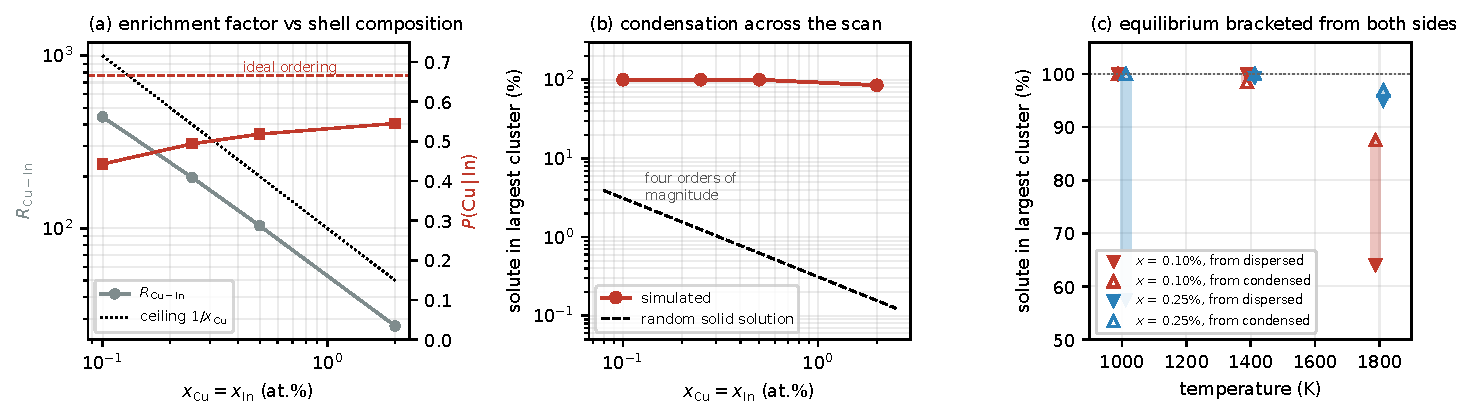
\includegraphics[width=\textwidth]{fig_condensation.pdf}
\caption{Equilibrium condensation at $L = 20$. (a)~The pair enrichment factor
$\RCuIn$ (grey, left axis) rises steeply on dilution, but only because its
ceiling $1/x_{\mathrm{Cu}}$ (dotted) rises faster; the copper content of the
first shell of indium (red, right axis) is nearly constant and approaches the
ideal ordered value of $2/3$ from below as the surface fraction falls.
(b)~Fraction of solute in the largest cluster, against the expectation for a
random solid solution at the same composition; the two differ by four orders of
magnitude. (c)~The bracketing test. At each temperature the state point is run
from a dispersed and from a pre-condensed configuration, which approach
equilibrium from opposite sides, so the equilibrium value lies within the shaded
interval. Filled triangles start dispersed, open triangles start condensed;
points are offset horizontally for clarity.}
\label{fig:cond}
\end{figure}

\subsection{The bracketing test}
\label{sec:bracket}

The results of Section~\ref{sec:scan} are subject to the objection that defeated
the earlier work. Two of the four state points achieved only two replica round
trips, and at 573~K the acceptance ratio within a replica is of order
$10^{-5}$. A configuration that has not equilibrated may be condensed simply
because it was quenched into a condensed basin, and no amount of additional
sampling at that temperature demonstrates otherwise if the sampler cannot cross
the barriers. \citet{yu2026} attempted to settle exactly this by propagating two
trajectories and observing that they converged on one another, and
Appendix~\ref{app:phase1} shows that this test returned a false positive: both
trajectories were metastable and their agreement carried no information.

We therefore do not rely on convergence at 573~K at all. Instead we exploit a
property of Markov chain dynamics that holds whether or not the chain has
converged: a chain started on one side of the equilibrium value approaches it
monotonically in distribution, so two chains started on \emph{opposite} sides
bracket it between them at all times. Each state point is run twice, once from a
random dispersed configuration and once from a pre-condensed configuration in
which all solutes occupy a single connected, charge-compensated domain
(Section~\ref{sec:protocols}). If the dispersed start aggregates and the
condensed start does not disperse, the equilibrium value lies between the two,
and this conclusion requires neither run to have converged.

The test is conducted at temperatures where the chain is demonstrably mobile
rather than at 573~K, and the bounding argument then transfers downwards:
because the ordered state becomes more strongly favoured relative to $k_BT$ as
temperature falls, condensation at any temperature below the tested range can be
no weaker than within it. Table~\ref{tab:bracket} gives the result.

\begin{table}[htbp]
\centering
\caption{Bracketing test at $L = 20$, 4000 sweeps per run. The entries give the
percentage of solute in the largest cluster reached from each starting
configuration; the equilibrium value lies between them. Acceptance ratios are
quoted to show that the chain is mobile at the upper temperatures.}
\label{tab:bracket}
\small
\begin{tabular}{rrrrrr}
\toprule
$x$ & $T$ (K) & acceptance & from dispersed & from condensed & equilibrium within \\
\midrule
0.10\,\% & 1800 & 0.094--0.119 & 64.1\,\% & 87.5\,\% & 64--88\,\% \\
0.10\,\% & 1400 & 0.007--0.012 & 100\,\%  & 98.4\,\% & 98--100\,\% \\
0.10\,\% & 1000 & 0.0004--0.0006 & 100\,\% & 100\,\% & 100\,\% \\
0.25\,\% & 1800 & 0.023--0.030 & 95.0\,\% & 96.9\,\% & 95--97\,\% \\
0.25\,\% & 1400 & 0.002--0.003 & 99.4\,\% & 100\,\%  & 99--100\,\% \\
0.25\,\% & 1000 & 0.0002--0.0003 & 57.5\,\%$^{\dagger}$ & 100\,\% & --- \\
\bottomrule
\end{tabular}

\vspace{2pt}
\begin{minipage}{0.92\textwidth}
\footnotesize $^{\dagger}$The single entry at which the two runs fail to
bracket usefully, and the one with the lowest acceptance in the table. It is
retained rather than omitted; see the text.
\end{minipage}
\end{table}

The pattern is unambiguous wherever the chain is mobile. At 1800~K, with
acceptance near 10\,\%, solutes starting dispersed \emph{spontaneously
aggregate} to between 64 and 95\,\% in a single cluster, and solutes starting
condensed \emph{do not disperse}. The bracket narrows and rises as temperature
falls: 64--88\,\% at 1800~K, 98--100\,\% at 1400~K, and 100\,\% at 1000~K
(Fig.~\ref{fig:cond}c).

Spontaneous aggregation from a dispersed start is the load-bearing observation.
A condensed configuration that merely fails to disperse could be kinetically
trapped; a dispersed configuration that assembles itself into a single domain,
at an acceptance ratio of 10\,\% where the chain is manifestly free to do
otherwise, cannot be. The two together close the argument from both sides.

One entry does not bracket. At $x = 0.25$~at.\% and 1000~K the dispersed start
reaches only 57.5\,\%, against 100\,\% from the condensed start, and this is
the lowest acceptance ratio in the table at $2\times10^{-4}$. The natural
reading is that the dispersed run has not had time to complete aggregation, so
its value is a lower bound rather than a bracket endpoint --- consistent with the
same composition reaching 99.4\,\% at 1400~K, where the chain moves an order of
magnitude faster. We retain the entry rather than omit it, since it marks
exactly where the method reaches its limit: bracketing is informative only while
both chains can move, and below that the argument must be carried by the
transfer downwards in temperature rather than by direct measurement.

\subsection{What has been established}
\label{sec:establishedcond}

Three statements follow, in decreasing order of strength.

The equilibrium state of this Hamiltonian at 0.10 and 0.25~at.\% is condensed,
established by bracketing at temperatures where the sampler is demonstrably
mobile, and transferred downwards to the ore-forming window by the monotonicity
of the ordering preference in $1/T$. This does not depend on any low-temperature
run having converged.

Complete condensation persists across a twentyfold range of composition in a box
eight times larger than that of \citet{yu2026}, with a monomer fraction of zero
throughout, against a random-solution expectation of 98\,\% monomers at the most
dilute point. The finite-size objection to the earlier result is therefore
answered.

The internal structure of the condensed domain is independent of bulk
composition to within the surface correction, so the object that forms is the
same object at every concentration examined, differing only in size.

What has \emph{not} been established is where, if anywhere, this behaviour
ceases. The compositions examined here span 0.10 to 2.00~at.\%, corresponding
to roughly 1000 to 20{,}000~ppm In, whereas most economically relevant
sphalerite carries tens to hundreds of ppm. How far downwards the behaviour
persists is taken up in Section~\ref{sec:limitations}, where an entropic
argument places the composition boundary well below natural tenors and the
simulations that would test that estimate are specified.

\section{Discussion}
\label{sec:discussion}

\subsection{Indium does not form a dilute solid solution}

The hypothesis stated in Section~\ref{sec:intro} was that under thermodynamic
equilibrium at ore-forming temperatures indium does not form a dilute solid
solution in sphalerite. Over the compositions accessible here, from 0.10 to
2.00~at.\%, it is confirmed, and the confirmation does not rest on the
convergence of any low-temperature simulation.

It is worth being precise about what a dilute solid solution would look like and
how far the observed state is from it. At $x_{\mathrm{In}} = 0.10$~at.\% a random
distribution of solutes over the cation sublattice leaves 97.6\,\% of them with
no solute among their twelve first neighbours, so such a solution would consist
almost entirely of isolated substituents, with a largest connected group of a
few atoms. The simulated equilibrium state has a monomer fraction of zero and a
largest cluster containing every solute in the box. These are not two points on
a continuum of ordering; they are different states of matter, separated by four
orders of magnitude in the relevant observable.

The physical origin is the pair binding energy of $-2\lambda$, which
\citet{yu2026} showed to be fixed by the dielectric constant of ZnS rather than
fitted, and which exceeds $k_BT$ at $300\,^\circ$C by a factor of twelve. A
dilute solid solution requires the configurational entropy of dispersal to
outweigh that binding energy. At 0.10~at.\% the entropy available per solute is of order
$k_B \ln(1/x_{\rm tot})$, where $x_{\rm tot} = 2x = 0.002$ is the total solute
fraction; this is $6.2\,k_B$, worth 0.31~eV at 573~K against a binding energy of
0.60~eV per Cu--In pair. Taking $x$ rather than $x_{\rm tot}$ raises the estimate
to $0.34$~eV and changes nothing. The comparison is not close, and it
becomes less close as temperature falls.

\subsection{Consequences for trace-element geochemistry}

\paragraph{Partition coefficients.} Indium partitioning between sphalerite and
hydrothermal fluid is conventionally modelled assuming ideal dilute mixing, with
configurational entropy $-k_B\sum_\alpha x_\alpha \ln x_\alpha$. If the
equilibrium state is condensed, that entropy is not available, and the indium
solubility inferred from such models is correspondingly too high. The size of
the error is not something the canonical simulations reported here can quantify,
because composition is fixed by construction; establishing it requires a
grand-canonical treatment in which the solute exchanges with a reservoir at
fixed chemical potential. We flag it as a target rather than claim a correction.

\paragraph{Enrichment factors in LA-ICP-MS datasets.} The artefact identified in
Section~\ref{sec:orderparamresult} is not confined to simulation. Any measure of
association normalised by bulk concentration --- an enrichment factor, a
correlation coefficient computed across samples of widely differing tenor, a
ratio of observed to expected co-occurrence --- has a ceiling set by that
concentration, and will appear to strengthen on dilution whether or not the
underlying association changes. In our data $\RCuIn$ rises sixteenfold across a
twentyfold dilution while the quantity it is meant to describe, the copper
content of the first shell around indium, falls slightly. Datasets spanning
orders of magnitude in trace-element content are precisely where this is most
available to be misread, and the remedy is to report the un-normalised
quantity alongside.

\paragraph{What a condensed state does and does not imply for analysis.} A
condensed equilibrium state means that indium in a sphalerite grain is not
expected to be uniformly distributed at the scale of the cation sublattice. It
does not follow that discrete inclusions must be resolvable, nor that bulk assay
is unrepresentative: the domains formed here contain $10^2$ to $10^3$ atoms and
are nanometric. What does follow is that micro-analytical mapping and bulk assay
measure different quantities in principle, and that the difference between them
carries information about the state rather than being analytical scatter.

\subsection{Sensitivity to the chemical term}
\label{sec:jsensitivity}

The conclusions above rest on a Hamiltonian containing one class of parameter,
$J_{\alpha\beta}$, that remains unconstrained by first-principles calculation.
We classify the conclusions accordingly.

\emph{Insensitive to $J$.} That the equilibrium state is condensed rather than
dilute does not depend on $J$. With all chemical terms switched off,
electrostatics alone enriches Cu--In first-neighbour bonds sixteenfold over the
random solid solution at $300\,^\circ$C and removes 96\,\% of the local charge
imbalance \citep{yu2026}; the pair binding energy of $-2\lambda$ that drives
condensation is fixed by the dielectric constant and contains no adjustable
parameter. Appendix~\ref{app:phase1} shows further that the electrostatic model
condenses more readily than the full model, not less, since its energy landscape
is smoother. Removing $J$ would therefore strengthen the central claim rather
than weaken it.

\emph{Sensitive to $J$.} The degree of ordering within the domain, the internal
Cu:In ratio, and any quantitative composition boundary do depend on $J$.
Switching $J$ on raises $\RCuIn$ from 16.0 to 25.0 at 2~at.\% and simultaneously
degrades local electroneutrality, driving the solute-shell Cu:In ratio from its
ideal value of 2.00 to 2.67. These are the quantities that an \textit{ab initio} determination of $J$ would
fix; Section~\ref{sec:dft} bounds them in the meantime.

\emph{A diagnostic that does not require knowing $J$ in advance.} Because
$\RCuIn$ and $\langle\dQ_a^2\rangle$ respond to $E_c$ in the same direction but
to $J$ in opposite directions, measurements sensitive to short-range order and
to local charge state --- EXAFS coordination numbers, XANES edge positions, or
bond-valence sums from high-resolution refinement --- can constrain the sign and
magnitude of the non-electrostatic term without a full \textit{ab initio}
calculation. Appendix~\ref{app:origin} identifies a third, independent
signature: the ruggedness of the energy landscape, observable as the replica
round-trip count at fixed computational cost.

\section{Limitations}
\label{sec:limitations}

We set these out in the order in which they bear on the central claim.

\paragraph{The composition range examined stops well above natural tenors.} The
scan spans 0.10 to 2.00~at.\%, roughly 1000 to 20{,}000~ppm indium, whereas most
economically relevant sphalerite carries tens to hundreds of ppm. The entropic
argument of Section~\ref{sec:discussion} favours condensation less strongly as
dilution proceeds, so a composition boundary must exist in principle, and this
work does not locate it. It establishes only that no such boundary lies within
the range examined.

The same argument can be pushed further, and the result is worth stating even
though it is an order-of-magnitude estimate rather than a measurement. Balancing
the dispersal entropy $k_B \ln(1/x_{\rm tot})$ against the energy a solute gains
on joining a domain, which is $2 n_b \lambda$ for a solute forming $n_b$
heterovalent bonds, gives
\begin{equation}
x_{\rm tot}^{\ast} \sim \exp\!\left(-\frac{2 n_b \lambda}{k_B T}\right).
\label{eq:solvus}
\end{equation}
At 573~K a solute joining the surface of a domain forms one or two heterovalent
bonds, and Eq.~\eqref{eq:solvus} then places the boundary between roughly
3~ppm and $10^{-5}$~ppm indium; a solute in a domain interior forms more, and the
estimate falls further still. Even the most conservative of these values lies at
or below the crustal abundance of indium, about 0.05~ppm, and all lie far below
the tens to hundreds of ppm carried by economically relevant sphalerite.

The implication, if the estimate survives direct calculation, is that no natural
sphalerite crystallises above the solvus. Every occurrence of indium in
sphalerite would then be supersaturated with respect to condensation, and the
question in any particular sample would never be whether the solute is disposed
to aggregate but only whether it has had time to. We flag this as a prediction
rather than a result: Eq.~\eqref{eq:solvus} neglects the entropy of the
condensed phase itself and treats $n_b$ as a constant. But it is a prediction
this framework makes, and the larger simulations described above would falsify
it if it is wrong.

Reaching tens of ppm is a question of hardware rather than of method. A box
holding a statistically meaningful number of solutes at 50~ppm requires of order
$5\times10^5$ cation sites, at which the calibrated ladder needs some tens of
replicas and a production run costs of order tens of core-days serially. The
implementation is verified correct at that box size
(Section~\ref{sec:verification}) and the scaling laws needed to plan such a
campaign are established (Section~\ref{sec:scaling}), so the obstacle is
computational rather than conceptual. All calculations reported here were
performed on a single workstation, which we regard as a feature: every result in
this paper can be reproduced on ordinary hardware. Locating the composition
boundary is left as a well-posed target for a parallel implementation, in which
replicas map naturally onto ranks with communication limited to an energy scalar
and an occasional configuration exchange.

\paragraph{The chemical term is not determined from first principles.}
Section~\ref{sec:jsensitivity} classifies which conclusions this affects and
Section~\ref{sec:dft} sets out what can be bounded without an \textit{ab initio}
calculation, but the quantitative statements about domain-internal ordering
should be read as conditional on the assumed values.

The obstacle is hardware and it is worth quantifying, because it defines what a
reader with an ordinary workstation can and cannot reproduce. The campaign of
Section~\ref{sec:dftplan} requires 216-atom supercells; at the plane-wave
cutoffs recommended for Zn, Cu, In and S the code's own estimate for a single
self-consistent calculation is 18.7~GB, against roughly 12~GB available on a
16~GB workstation.
Reducing the cutoff far enough to fit would degrade precisely the energy
differences the campaign exists to measure, since those differences are small
relative to the total energies. The structures, input files and fitting harness
are nonetheless released and validated, so the calculation can be run by anyone
with sufficient memory and the parameters dropped into the model without
repeating any of the sampling reported here.

\paragraph{Iron is absent.} Natural sphalerite commonly carries up to 10~mol\%
FeS. $\mathrm{Fe^{2+}}$ is isovalent with $\mathrm{Zn^{2+}}$ and so does not
enter the charge-compensation term at all, but it modifies the dielectric
response that fixes $\lambda$, and direct $J_{\mathrm{Fe\text{-}In}}$ and
$J_{\mathrm{Fe\text{-}Cu}}$ terms need not vanish. Whether this matters is
itself a measurable question, framed in Section~\ref{sec:dftplan} and subject to
the same hardware constraint.

\paragraph{The treatment is rigid-lattice and athermal in its elasticity.}
Atomic relaxation enters only through continuum expressions, which
\citet{yu2026} showed to be numerically negligible for Cu--In because the size
mismatch is small; the same would not hold for substituents with large misfit,
and the framework should not be transferred to those without re-examination.

\paragraph{Monte Carlo sweeps are not physical time.} Nothing in this work
constrains the rate at which equilibrium is approached in a cooling ore body.
The bracketing construction of Section~\ref{sec:bracket} establishes what the
equilibrium state \emph{is}; whether a natural sphalerite grain attains it
depends on diffusion rates and cooling history, and multi-domain configurations
in natural samples are expected to reflect exactly that gap. That question is
outside the scope of this paper and is treated separately.

\section{Conclusions}
\label{sec:conclusions}

\begin{enumerate}\itemsep3pt
\item Under the configurational Hamiltonian of \citet{yu2026}, the equilibrium
      state of indium in sphalerite at ore-forming temperatures is condensed,
      not a dilute solid solution, at every composition examined between 0.10
      and 2.00~at.\%. The monomer fraction is zero throughout, against a
      random-solution expectation of 98\% at the most dilute point.

\item This is not a finite-size artefact. The same 160 solute atoms that
      exhausted the box of the preceding study condense completely in eight
      times the volume, and halving the concentration again, so that each solute
      has five hundred sites of room, does not change the outcome.

\item The result does not rest on converging any low-temperature simulation.
      Running each state point from a dispersed and from a pre-condensed
      configuration brackets the equilibrium value between two approaches from
      opposite sides, and the transfer to lower temperature follows from the
      monotonicity of the ordering preference in $1/T$.

\item The pair enrichment factor is a misleading observable in the dilute limit,
      since its ceiling is $1/x_{\rm Cu}$. Cluster-size distributions and
      un-normalised shell compositions should be reported instead, in simulation
      and in analytical datasets alike.

\item Condensation is driven by electrostatics and does not depend on the
      unconstrained chemical term. Removing that term strengthens the conclusion,
      because the resulting energy landscape is smoother and the system condenses
      more readily.

\item The ideal dilute-mixing entropy assumed in conventional
      partition-coefficient models is not available if the equilibrium state is
      condensed, so indium solubilities inferred from such models are too high.
      Quantifying the correction requires a grand-canonical treatment.

\item What remains open is where this behaviour ceases. Natural tenors run an
      order of magnitude below the compositions reached here, and locating a
      composition boundary requires boxes of order $5\times10^5$ sites. The
      implementation is verified correct at that scale and the scaling laws are
      established; the obstacle is computational, not conceptual.
\end{enumerate}

%==============================================================================
\appendix
\section{The equilibration correction to \citet{yu2026}}
\label{app:phase1}

\subsection{What was claimed}

\citet{yu2026} addressed the possibility that the low-temperature plateau in
their order parameters was a consequence of configurational freezing rather than
thermodynamic saturation. Their test propagated two trajectories at 573~K, one
quenched directly from a random configuration and one pre-annealed through 2000,
1400, 1000 and 800~K. The two converged to $\aInCu = -23.17$ and $-23.48$
respectively, a difference of 1.3\,\%, with both order parameters stationary over
the final $1.2\times10^4$ sweeps, and the paper concluded that the plateau was
thermodynamic in origin.

\subsection{Why the test could not support that conclusion}

Applying replica exchange to the same Hamiltonian, box and composition, with an
adaptively calibrated ladder, gives $H/N = -0.00605$~eV per site from a quenched
start within the same total sweep budget that leaves plain Kawasaki dynamics at
$-0.00271$~eV. That is 0.77~meV per site, or 3.1~eV over the box, below the
pre-annealed trajectory, which was the lowest state the earlier work reached.
The result is reproduced by independent runs with different seeds, ladder
lengths and exchange frequencies; five such configurations agree on the energy
to 0.055~meV per site.

Both trajectories of the original test were therefore metastable, and their
agreement with one another carried no information about equilibrium. The
metastability that the earlier work did report --- 3.2~meV per site between the
quenched and annealed states --- was real, but it was itself an underestimate of
the distance to equilibrium.

The general lesson is transferable and is the reason this appendix is included
rather than confined to an erratum. \emph{In a system whose acceptance ratio is
of order $10^{-5}$, the convergence of two trajectories towards each other is
not a test of equilibration.} Two chains launched into the same basin will
agree with each other whether or not that basin is the equilibrium one. What is
required is a sampler capable of crossing the barriers, together with a
diagnostic that measures whether it is actually doing so --- for replica
exchange, the round-trip count of Section~\ref{sec:roundtrips}. It is precisely
because this failure mode is silent that the present paper rests its central
claim on the bracketing construction of Section~\ref{sec:bracket}, which
requires no run to have converged.

\subsection{Corrected values, and what they change}

Table~\ref{tab:correction} gives the corrected values at 573~K.

\begin{table}[htbp]
\centering
\caption{Values at 573~K for the full model of \citet{yu2026}, as originally
reported from the annealing protocol and as re-measured by replica exchange.}
\label{tab:correction}
\small
\begin{tabular}{lrrr}
\toprule
& annealing & replica exchange & shift \\
\midrule
$H/N$ (eV per site)          & $-0.00528$ & $-0.00605$ & $-0.00077$ \\
$\aInCu$                      & $-23.48$   & $-24.00$   & $2.2$\,\% \\
$\RCuIn$                      & $24.48$    & $25.00$    & $2.1$\,\% \\
$\langle\dQ_a^2\rangle$       & $0.0120$   & $0.0100$   & $-17$\,\% \\
charge imbalance removed      & $92.4$\,\% & $93.7$\,\% & --- \\
solute clusters               & 1 (160 atoms) & 1 (160 atoms) & unchanged \\
In first shell, Cu\,/\,In\,/\,Zn & 0.490\,/\,0.183\,/\,0.327
                               & 0.500\,/\,0.188\,/\,0.312 & --- \\
\bottomrule
\end{tabular}
\end{table}

The order parameters shift by about 2\,\%, in the direction of insufficient
ordering, as under-convergence requires. No conclusion of the earlier work is
altered by the correction.

Two consequences bear on the present paper. First, the solute-shell composition
Cu:In moves only from 2.68 to 2.67 against the ideal 2.00, so the departure from
ideal ordering identified there is a real feature of the Hamiltonian and not a
sampling artefact. Second, and more useful, the correction is confined to the
full model: the electrostatics-only calculation, re-measured with a ladder built
for that Hamiltonian and a production run achieving thirteen round trips,
returns $\aInCu = -14.99$, $\RCuIn = 15.99$ and
$\langle\dQ_a^2\rangle = 0.0065$ --- the published values, to every digit
reported. Four independent ladders with tops at 2000, 2400, 2800 and 3000~K and
lengths of 20 to 29 replicas agree on the energy to 0.001~meV per site.

\subsection{Where the sampling difficulty comes from}
\label{app:origin}

The two Hamiltonians differ only in $J_{\alpha\beta}$, so that contrast
localises the difficulty precisely: the sampling problem is caused by the
hypothetical covalent term, not by the charge-compensation term. On the pure
$E_c$ landscape the system anneals to equilibrium without difficulty; adding $J$
makes it rugged. The same run achieves thirteen replica round trips for the
electrostatic model against five for the full model at equal computational cost.

The mechanism is visible in the bond census. At fixed composition the
configurational part of $E_c$ is
$2\lambda \sum_{\langle ij\rangle} \delta q_i \delta q_j$, so $E_c$ is minimised
by maximising the excess of heterovalent over homovalent solute contacts. The
electrostatic model does exactly that, forming an open network with 307 Cu--In
bonds and \emph{no} homovalent solute contacts whatever. The full model instead
has 480 Cu--In bonds together with roughly 90 Cu--Cu and 90 In--In, buying a
56\,\% denser Cu--In network at the cost of 4.2~eV of electrostatic energy. The
homovalent contacts are not something $J$ tolerates but something the denser
packing forces: the fcc cation sublattice contains 24 triangles through every
site, so a compact solute domain cannot be two-coloured without homovalent
edges. The competition between $E_c$, which favours an open alternating network,
and $J$, which favours dense aggregation, is what makes the full-model landscape
rugged.

This has a practical implication, taken up in Section~\ref{sec:dft}. The ruggedness of
the energy landscape, observable as the round-trip count at fixed computational
cost, is a third signature of $J$ alongside $\RCuIn$ and
$\langle\dQ_a^2\rangle$, and unlike those two it is a property of the dynamics
rather than of the equilibrium state.

\section{Supplementary sampling diagnostics}
\label{app:sampling}

\subsection{Move sets that do not work}

Two natural-looking modifications of the sampler were tried and failed, in ways
that are informative rather than merely negative.

\paragraph{Boosted solute--solute exchange.} In the proposal of
\citet{yu2026} the partner site is drawn uniformly from all $N$ sites, so at
2~at.\% substitution only 4\% of trial moves exchange two solutes. Since the
slow mode identified there was the reordering of a domain interior, and since a
Cu $\leftrightarrow$ In swap reorders the interior without breaking any Cu--In
bond, raising that fraction seemed an obvious improvement. It is not: measured
in a single replica at 573~K, the acceptance of solute--solute exchange is
exactly zero. Swapping a Cu for an In inside an ordered domain destroys the
local charge-compensation pattern at a cost of order $4\lambda$, which against
$k_BT = 0.049$~eV is unreachable. The move becomes useful only inside replica
exchange, where hot replicas accept it freely and pass decorrelated
configurations down the ladder; we retain it at $p_{ss} = 0.5$ for that reason
alone.

\paragraph{Cluster algorithms.} A Wolff or Swendsen--Wang construction does not
apply here, for two independent reasons. The pair coupling
$2\lambda\,\delta q_i \delta q_j$ changes sign with the species pair --- negative
for heterovalent contacts, positive for homovalent ones --- so the model is
sign-frustrated and the Fortuin--Kasteleyn mapping that underpins those
algorithms does not hold. Separately, cluster flips do not conserve composition,
which the canonical ensemble requires. The appropriate generalisation is the
geometric cluster algorithm \citep{dress1995,liu2004}, which conserves
composition by construction; we have not implemented it.

\subsection{Why round trips and not acceptance}

Table~\ref{tab:rt} records the experiment behind the recommendation of
Section~\ref{sec:roundtrips}. All five configurations were run at identical
computational cost.

\begin{table}[htbp]
\centering
\caption{Replica round trips at fixed compute, $L = 10$, 573~K.}
\label{tab:rt}
\small
\begin{tabular}{rrrrr}
\toprule
$M$ & sweeps per exchange & ladder top (K) & round trips & median swap acceptance \\
\midrule
29 & 5 & 3000 & 0  & 0.576 \\
29 & 2 & 3000 & 3  & --- \\
29 & 1 & 3000 & 7  & 0.582 \\
21 & 1 & 2600 & 12 & --- \\
19 & 1 & 2200 & 13 & --- \\
\bottomrule
\end{tabular}
\end{table}

Attempting exchanges after every sweep rather than every five takes the
round-trip count from zero to seven while the median swap acceptance moves by
less than 0.01. A study reporting acceptance alone would have seen nothing, and
would have concluded that its ladder was performing well while no replica was
traversing it. Lowering the ladder top from 3000 to 2200~K compounds the
improvement, requiring ten fewer replicas and reaching thirteen round trips: the
replicas above 2400~K were buying nothing, because the system is fully
disordered well below 3000~K. All five configurations agree on the internal
energy at 573~K to 0.055~meV per site, so the equilibrium value is
protocol-independent even where the round-trip statistics are not.

\subsection{Verification at scale}

The implementation was verified at $L = 10, 20, 30, 40$ and $50$, that is up to
$N = 5\times10^5$ cation sites. The checks are: reciprocity of the adjacency
tables; the sharing property of Section~\ref{sec:background}, tested on random
samples of sites at each box size rather than at a single reference site;
agreement between the incrementally accumulated energy and a full recomputation
\emph{after} a production-length run, which exposes accumulated drift (observed
relative deviation $<10^{-9}$); exact conservation of composition; integrity of
the solute index list under solute--solute exchange; and the random-solution
limits $R \to 1$, $R = 1 - \alpha$ and $\langle\dQ_a^2\rangle = 8x$. All pass at
every box size.

Throughput falls as $N^{-0.217}$, reaching 37\% of the small-box rate at $50^3$
($1.37\times10^6$ trial moves per second, 0.366~s per sweep, single core),
because the partner site is drawn uniformly from all $N$ sites and the adjacency
arrays leave cache above $N \sim 10^5$. Memory is not the constraint: 64~MB of
adjacency tables shared across replicas, 4.7~MB per replica.

%==============================================================================
\section*{Data and code availability}
\label{sec:availability}
Source code, numerical results and figures for this study are openly available
at \url{https://github.com/Ruqing1963/sphalerite-equilibrium-mc}. Code is
released under the MIT licence and data under CC~BY~4.0; the manuscript remains
the copyright of the authors. The repository includes the verification suite
that reproduces every analytic limit quoted here, the adaptive ladder
construction, the scripts that regenerate each figure, and the structure
generation and fitting harness for the parameterisation campaign of
Section~\ref{sec:dftplan}, so that the latter can be run by anyone with
sufficient memory and the parameters dropped into the model without repeating
any of the sampling reported here.

The lattice model itself, together with the analytic results recapitulated in
Section~\ref{sec:background}, is archived separately with
\citet{yu2026} at \url{https://github.com/Ruqing1963/sphalerite-lattice-mc}.

\section*{Funding}
This study was funded by the Hezhou Municipal Scientific Research and
Development Program (Project Nos.\ 2024143, 2024141 and 2024104).

%==============================================================================
\begin{thebibliography}{99}
\itemsep2pt

\bibitem[Dress and Krauth(1995)]{dress1995}
Dress, C., Krauth, W. (1995) Cluster algorithm for hard spheres and related
systems. \textit{Journal of Physics A} 28, L597--L601.

\bibitem[Liu and Luijten(2004)]{liu2004}
Liu, J., Luijten, E. (2004) Rejection-free geometric cluster algorithm for
complex fluids. \textit{Physical Review Letters} 92, 035504.

\bibitem[Moura et al.(2007)]{moura2007}
Moura, M.A., Botelho, N.F., de Mendon\c{c}a, F.C. (2007) The indium-rich
sulfides and rare arsenates of the Sn-In-mineralized Mangabeira A-type granite,
central Brazil. \textit{The Canadian Mineralogist} 45, 485--496.

\bibitem[USGS(2024)]{usgs2024}
U.S. Geological Survey (2024) \textit{Mineral Commodity Summaries 2024:
Indium}. U.S. Geological Survey, Reston, Virginia.

\bibitem[Werner et al.(2015)]{werner2015}
Werner, T.T., Mudd, G.M., Jowitt, S.M. (2015) Indium: key issues in assessing
mineral resources and long-term supply from linchpin polymetallic deposits.
\textit{Applied Earth Science} 124, 213--226.

\bibitem[Yu et al.(2026)]{yu2026}
Yu, H., Chen, R., Lu, H. (2026) A statistical thermodynamic lattice model for
Cu--In coupled substitution in sphalerite, version 2.0. \textit{Zenodo}.
\url{https://doi.org/10.5281/zenodo.21880502}

\end{thebibliography}

\end{document}
